\documentclass{SGGW-thesis-EN}
\usepackage[utf8]{inputenc}
\usepackage[backend=biber,style=numeric]{biblatex}
\usepackage{tabularx}
\usepackage{tikz}
\usepackage{listings}
\usepackage{xcolor}
\usepackage{booktabs}


\lstdefinelanguage{yaml}{
  keywords={true,false,null,yes,no},
  keywordstyle=\color{blue},
  basicstyle=\ttfamily\small,
  sensitive=false,
  comment=[l]{\#},
  morecomment=[l]{\#},
  morestring=[b]",
  morestring=[b]'
}
\usetikzlibrary{positioning, arrows.meta, shapes.geometric}
\addbibresource{references.bib}

\MASTERtrue
\WZIMtrue

\title{Automated Extraction and Categorization of Product Information from Receipts}
% command \Ptitle{} can be used to give the title in Polish, if this is necessary, and can be deleted if you do not need the title in Polish
\Ptitle{}
\author{Michał Zaręba}
\date{2017}
\album{196218}
\thesis{Diploma thesis in the field of}
\course{Information Science}
\promotor{dr hab.\ inż.\ Leszek Chmielewski, prof.\ SGGW}
\pworkplace{Institute of Information Technology\\Department of Artificial Intelligence}

\usepackage{hyperref}

\begin{document}
\maketitle
\statementpage
% titles and abstracts must be given in two languages - PL, EN
\abstractpage
{Extraction and categorization}
{}
{OCR, BERT, Transformer, NLP, thesis, implementation, SGGW, Warsaw University of Life Sciences}
{Ekstracja i kategoryzacja }
{lorem ipsum}
{OCR, BERT, Transformer, NLP, thesis, implementation, SGGW, Warsaw University of Life Sciences}



\tableofcontents


\startchapterfromoddpage % niezależnie od długości spisu treści pierwszy rozdział zacznie się na nieparzystej stronie

\chapter{Introduction}

\section{Motivation}
Tracking of expenses and managing personal finances is an important aspect of modern life.
With an increasing number of daily transactions and a vast variety of products available, individuals face significant challenges in effectively monitoring their spending and managing their budgets. 
Although receipts contain valuable details that could help consumers analyze and control their expenses, 
the majority of consumers either discard receipts shortly after purchase or find it too tedious and time-consuming to analyze them manually. 
Automating the extraction and categorization of product information from receipts could significantly simplify budget tracking and provide insights into spending habits, enabling consumers to understand precisely where their money goes.
Simple and efficient way to track expenses is essential for individuals who wish to maintain a clear overview of their spending habits and make informed financial decisions. 


\section{Problem Statement}
Most existing expense-tracking solutions focus primarily on invoices, bank statements, or require manual input. 
Large corporations and organizations typically possess the necessary budgets and technical resources to implement robust, 
automated systems for extracting and categorizing expense data from structured documents such as invoices or bank statements. 
For personal use, however, the most commonly available and practical source of spending information remains paper receipts. 
Current receipt-based solutions are often limited: many tools available today are either designed exclusively for commercial purposes, 
lack support for languages other than English, or are inadequately trained to accurately process Polish-language receipts.  
Thus, there is a clear gap and a significant need for a solution that effectively automates extraction and categorization of product details from receipts, 
specifically accommodating the complexity and linguistic characteristics of the Polish language.

\section{Objectives of the Study}
This study has two primary objectives, each directly addressing the challenges identified in the problem statement:

\begin{enumerate} 
  \item Develop a robust system capable of automatically extracting structured product information (such as product names, and prices) from Polish-language receipts using Optical Character Recognition (OCR).
  \item Implement and evaluate a product categorization module based on the embeddings generated by pre-trained models, specifically BERT (Bidirectional Encoder Representations from Transformers),
  and Sentence-BERT model (Siamese transformer network) fine-tuned with own data. 
  \item The extracted embeddings serve as input to an XGBoost classifier responsible for categorizing products into predefined expense-related categories.
\end{enumerate}

These objectives will be thoroughly addressed and analyzed in subsequent chapters. 
Given the complexity of Polish-language receipts and limited availability of labeled datasets, achieving optimal results will require careful integration and fine-tuning of multiple technologies. 
Critical aspects will include the effective integration of OCR and NLP components, as well as the development of a robust classification model capable of accurately categorizing products based on their textual descriptions that might
often be ambiguous, multiple-worded, or contain spelling errors.
\newpage
\section{Scope and Limitations}

The scope of this study is limited to the development of a system capable of automatically extracting product information from receipts and categorizing these products into predefined categories. 
The system specifically targets Polish-language receipts and will be evaluated primarily on its ability to accurately extract product costs and perform correct product categorization.

\noindent \\The limitations of this study include the following:

\begin{itemize}
    \item The developed system will not include additional functionalities such as expense tracking over time, financial report generation, or integration with external personal financial management tools.
    \item The scarcity of comprehensive, labeled Polish-language receipt datasets restricts the potential accuracy and generalization capabilities of the models developed. Consequently, results may vary when encountering receipt formats or text variations not present in the training data.
    \item The OCR will be employed without utilizing spatial information or context regarding the positioning of text on receipts. Therefore, preprocessing steps such as image cropping, alignment, and noise reduction are necessary to ensure the OCR engine receives properly formatted and isolated textual inputs.
\end{itemize}

\chapter{Literature Review}

\section{Optical Character Recognition (OCR) Technologies}
Optical Character Recognition (OCR) refers to the process of converting textual information from scanned or photographed images into machine-readable formats. 

Traditional OCR techniques primarily relied on template matching, statistical classification, and structural analysis, with limited adaptability to varying fonts and noisy inputs.\cite{ocrsystems}

Modern OCR systems use deep learning models that typically combine convolutional neural networks (CNNs) for feature extraction with recurrent or attention-based architectures (e.g., LSTM, GRU) for sequence modeling. This architecture enables the system to learn complex patterns and recognize characters across varying fonts, sizes, and orientations \cite{shi2016endtoend}.

Recent OCR models further incorporate attention mechanisms, allowing the network to dynamically focus on relevant regions of the input image. Unlike standard OCR models, LayoutLM introduces explicit spatial awareness by incorporating positional embeddings of text regions, which is particularly effective for structured documents like receipts \cite{li2020layoutlm}.
While attention-based models with spatial awareness offer notable improvements in accuracy and robustness, their effectiveness remains constrained by the availability of large, annotated datasets. As a result, the OCR systems evaluated in this study—Tesseract and PaddleOCR—do not model document structure explicitly and operate at the text-line level.

Tesseract is an open-source OCR engine maintained by Google, widely adopted across various applications. It supports multiple languages, including Polish, and can be fine-tuned on domain-specific datasets for improved accuracy. Since version 4.0, it incorporates an LSTM-based recognition engine, enhancing its performance on noisy or multilingual documents \cite{smith2007overview, smith2013history}. Tesseract is highly configurable, offering control over segmentation modes, character whitelists, and language models. Fine-tuning involves training on a targeted dataset, which can significantly enhance accuracy for specific formats such as Polish receipts.
\newpage
PaddleOCR is a deep learning-based OCR framework developed by Baidu, supporting over 80 languages. The framework proposes a OCR system,
that is modular and made of text detection, detected boxes rectification and text recognition. Thanks to the use of a several augmentation techniques, PaddleOCR achieves a balance between accuracy and speed, 
making it suitable for real-time applications and mobile devices.

Text detection is handled using Differentiable Binarization that is a segmentation network. Simplicity of the model combined with minor postprocessing
holds the effectiveness of this module. Then the detected boxed are rectified using a text direction classifier and fed into a text recognition model.
The text recognition model is based on a CRNN architecture, specifically designed for recognizing characters in images. 
It employs a combination of convolutional layers and recurrent layers to capture both local and sequential features of the text. 
For further enchancement several strategies are used, such as light backbone or data augmentation \cite{du2020ppocr}. 

\begin{figure}[h!]
  \centering
  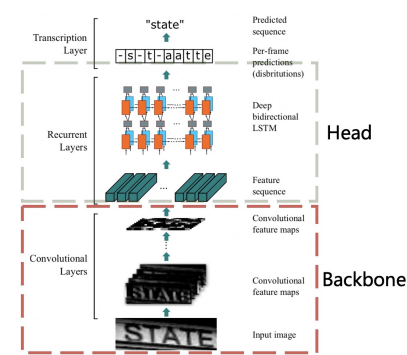
\includegraphics[width=1\textwidth]{images/cnn_text_recognizer.png}
  \caption{CRNN text recognition architecture. \cite{shi2015e2etnn}}
  \label{fig:cnn_text_recognizer}
  \end{figure}
\begin{figure}[h!]
  \centering
    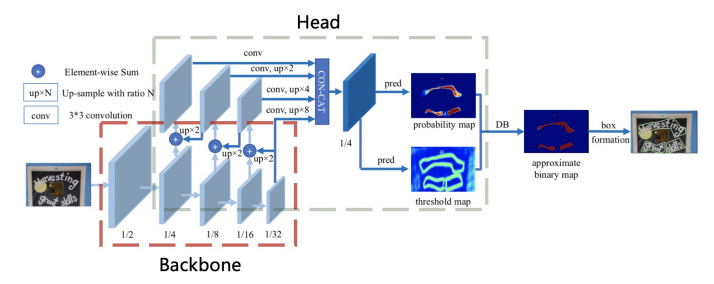
\includegraphics[width=1\textwidth]{images/text_detector_db.png}
    \caption{DBNet text detection architecture. \cite{liao2019rttextdet}}
    \label{fig:text_detector_db}
  \end{figure}

\newpage
\section{Semantic Text Embeddings for Receipt Item Categorization}
To enable machine learning models to analyze text, the text must first be converted into a numerical format—a process known as vectorization or word embedding which is a crucial step in Natural Language Processing (NLP).
Word embeddings are fixed-length vector representations that encode the semantic meaning of words and the relationships between them. 
The words with similar meanings are represented by similar vectors in the embedding space.\cite{almeida2023wordembeddingssurvey}

\begin{figure}[h!]
  \centering
    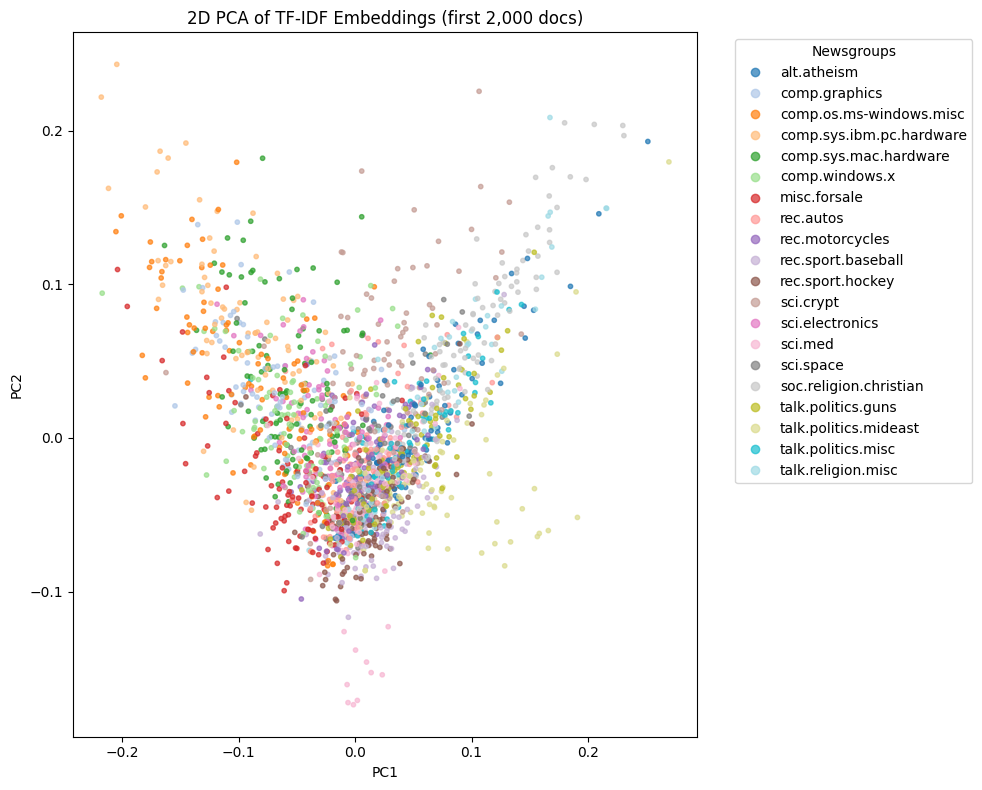
\includegraphics[height=9cm]{images/tfidf_embeddings.png}
    \caption{TF-IDF embeddings on News Groups dataset from scikit-learn.}
    \label{fig:tfidf_embeddings}
  \end{figure}

\newpage 
There are several approaches to generating these embeddings, and this section outlines the most common methods, explaining how they work and highlighting their key differences.
Prior to embedding, text must be preprocessed. This includes normalization steps such as lemmatization or stemming, and tokenization, which segments text into individual words or tokens \cite{jurafsky2023slp3}.
After those we can proceed to several methods of generating word embeddings, which can be broadly categorized into two groups: count-based and prediction-based methods, and will be described below.

\subsection{Count-based Methods}
Count-based methods rely on the idea that the meaning of a word can be inferred from its co-occurrence with other words in a given context.
Those methods typically involve creating a sparse matrix, where each row and column represents a word in the vocabulary, and the values in the matrix represent the frequency of co-occurrence between pairs of words.
The two most common approaches are the Bag of Words (BoW) and Term Frequency-Inverse Document Frequency (TF-IDF)\cite{jurafsky2023slp3}.

Bag of words represents a document as an unordered vector of word counts, ignoring the order of words and their grammatical relationships.

TF-IDF model, on the other hand, assigns weights to words based on their frequency in a document relative to their frequency in the entire corpus. 
This helps to highlight important words that are more informative for the specific document.

\subsection{Prediction-based Methods}
Prediction-based methods are word representation techniques that learn embeddings by predicting words from context (or vice versa), unlike count-based methods which rely on raw frequency statistics.
The two most common prediction-based methods are Word2Vec and BERT which are based on neural networks and their representation of words is contained in dense matrix different from the sparse matrix used in count-based methods.
The dense matrixes turns out to be more efficient and effective for representing the meaning of words in a lower-dimensional space.\cite{jurafsky2023slp3}

Word2vec is a framework used for calculating a static embeddings, that mean there is a certain numerical representation for each word in vocabulary.
There are two architectures for training Word2Vec models: Continuous Bag of Words (CBOW) and Skip-Gram.
\begin{enumerate}
  \item \textbf{Continuous Bag of Words (CBOW)}: predicts the target word from surrounding context words.
  \item \textbf{Skip-Gram} Skip-Gram: predicts context words from a single target word.
\end{enumerate}
Skip-Gram is particularly effective for representing rare words, as it captures word–context associations more accurately,
whereas CBOW offers greater computational efficiency and faster training times \cite{mikolov2013distributed}.

\textbf{BERT (Bidirectional Encoder Representations from Transformers)} is a deep learning model introduced by Google that generates contextualized word embeddings by processing text in both directions (left-to-right and right-to-left) simultaneously. 
Unlike earlier models that produce static embeddings, BERT captures the meaning of a word based on its entire sentence context. 
Transformer architecture, the backbone of BERT, employs self-attention mechanisms to weight the importance of words in relation to each other, allowing the model to derivate complex semantic relationships between them.
To achieve this, BERT is pretrained using a two-step self-supervised training process:
\begin{enumerate}
  \item \textbf{Masked Language Model (MLM)}: Randomly masks a percentage of input tokens and trains the model to predict the masked words based on context.
  \item \textbf{Next Sentence Prediction (NSP)}: Trains the model to predict whether two sentences are follow each other or not, improving its understanding of sentences coherence.
\end{enumerate}

\begin{figure}[h!]
  \centering
    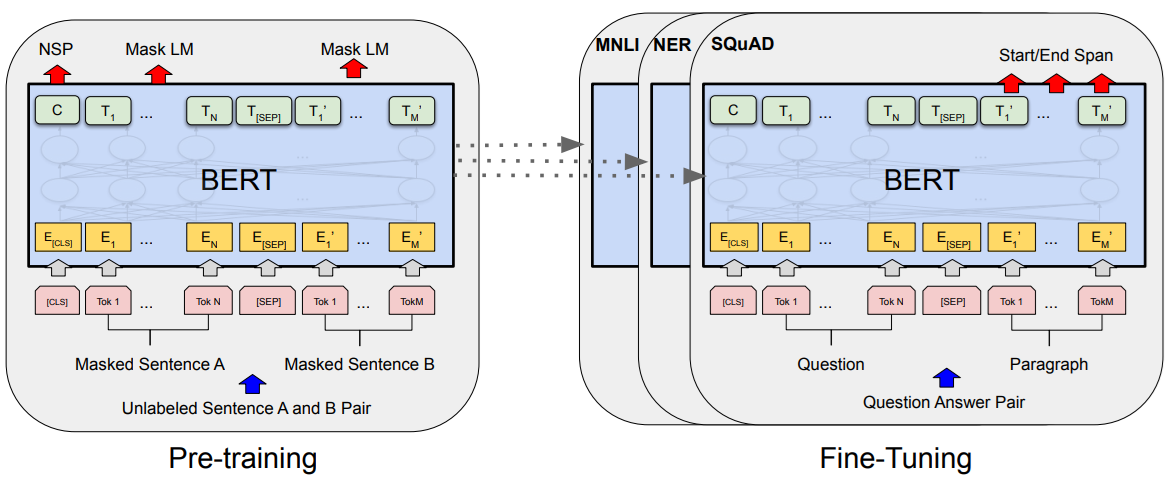
\includegraphics[height=5cm]{images/bert_procedures.png}
    \caption{BERT training procedures \cite{devlin2019bertpretrainingdeepbidirectional}}
    \label{fig:bert_procedures}
  \end{figure}

These context-aware embeddings have demonstrated strong performance across various NLP tasks, including classification.\cite{devlin2019bertpretrainingdeepbidirectional}.
In this study, embeddings generated by pre-trained BERT models serve input features for classification task which will categorize products into predefined expense-related categories.


\section{XGBoost Classifier}
XGBoost (eXtreme Gradient Boosting) is an open-source machine learning library implementing the gradient boosting framework, 
primarily with decision trees. It is a state-of-the-art supervised learning algorithm known for consistently achieving top performance across numerous machine learning challenges \cite{Chen_2016}.

Gradient boosting is an ensemble learning technique that instead of training a single model, build an initial simple model 
and then iteratively fits new models to  minimize the loss function\cite{natekin2013gradient}.

The XGBoost model employs several specific techniques to enhance its predictive capabilities:
\begin{enumerate}
  \item Regularization: Prevents the creation of overly complex trees, thereby minimizing overfitting and improving generalization.
  \item Gradient Tree Boosting with second-order Taylor approximation: Incorporates both first-order (gradient) and second-order (Hessian) derivatives of the loss function, significantly improving estimation accuracy and computational efficiency.
  \item Shrinkage (learning rate): After each boosting step, prediction scores are scaled by a small factor (learning rate). This regularization strategy prevents overfitting and ensures the model learns gradually and robustly.
  \item Column subsampling: Inspired by random forests, this technique randomly selects subsets of features when building each tree, further reducing overfitting and enhancing training efficiency. 
\end{enumerate}
XGBoost uses an ensemble of decision trees to make predictions. 
Each tree in this ensemble contributes to the final prediction by adding its own output to the outputs of all previous trees.

Mathematically, the final prediction $\hat{y}_i$ for an instance $x_i$ is given by:

\begin{figure}[h!]
  \centering
  \begin{minipage}[c]{0.4\textwidth}
      \centering
      \[
      \hat{y}_i = \sum_{k=1}^{K} f_k(x_i)
      \]
  \end{minipage}\hfill
  \begin{minipage}[c]{0.55\textwidth}
      \centering
      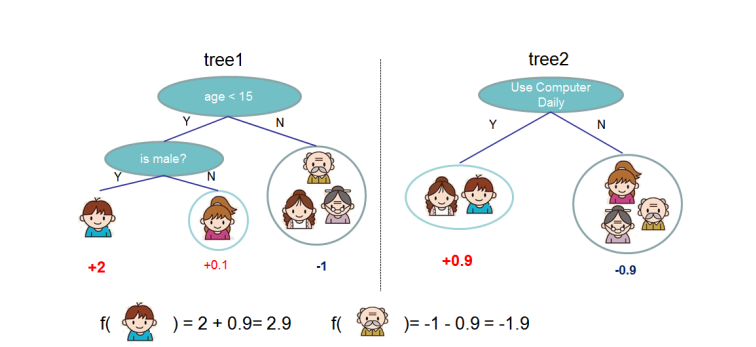
\includegraphics[width=\linewidth]{images/tree_ensemble_model.png}
      \caption{Tree ensemble model \cite{Chen_2016}}
      \label{fig:tree_ensemble_model}
  \end{minipage}
\end{figure}
To train these trees effectively, XGBoost optimizes a simplified objective function derived using second-order approximations (gradients and Hessians). 
This objective helps determine the optimal structure and weights of each tree. The simplified final objective at each iteration is expressed as:

\begin{figure}[h!]
  \centering
  \begin{minipage}[c]{0.4\textwidth}
      \centering
    \[
    \tilde{L}^{(t)}(q) = -\frac{1}{2}\sum_{j=1}^{T}\frac{(\sum_{i \in I_j} g_i)^2}{\sum_{i \in I_j} h_i + \lambda} + \gamma T
    \]
  \end{minipage}\hfill
  \begin{minipage}[c]{0.55\textwidth}
      \centering
      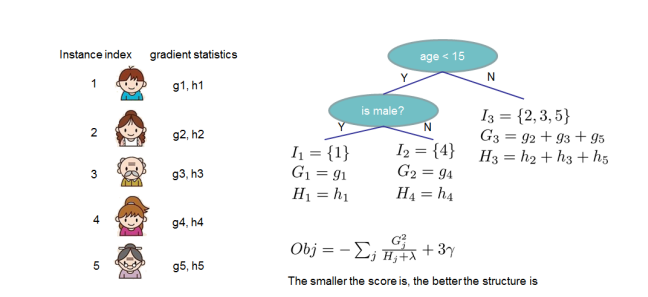
\includegraphics[width=\linewidth]{images/Structure score calculation.png}
      \caption{Structure Score Calculation \cite{Chen_2016}}
      \label{fig:Structure_score_calculation}
  \end{minipage}
\end{figure}
Here, $g_i$ and $h_i$ represent gradient statistics, indicating how predictions should change to minimize the error. The terms $\gamma$ and $\lambda$ are hyperparameters that penalize complex trees to prevent overfitting.
Hyperparameters are parameters defined before training, which control the learning process.  
In XGBoost, these hyperparameters significantly affect how the model is trained and how it performs.
\begin{table}[h!]
  \centering
  \caption{XGBoost Hyperparameters and Their Roles}
  \label{tab:xgboost_hyperparameters}
  \begin{tabularx}{\textwidth}{|l|X|}
  \hline
  \textbf{Hyperparameter} & \textbf{Role and Effect} \\ \hline
  \texttt{learning\_rate} & Controls the rate at which the model learns. Lower values reduce overfitting but require more trees. \\ \hline
  \texttt{max\_depth} & Limits the depth of the trees. Greater depth increases model complexity and the risk of overfitting. \\ \hline
  \texttt{n\_estimators} & Determines the total number of trees in the ensemble. Increasing trees usually enhances performance but extends training time. \\ \hline
  \texttt{subsample} & The fraction of samples randomly chosen to build each tree. Lower values help reduce overfitting. \\ \hline
  \texttt{colsample\_bytree} & The fraction of features randomly selected to build each tree, reducing correlations between trees and preventing overfitting. \\ \hline
  \texttt{min\_child\_weight} & Minimum sum of instance weights in a child node. Higher values encourage simpler, less detailed trees, reducing overfitting. \\ \hline
  \texttt{gamma} & Minimum required loss reduction for creating new splits. Higher values lead to simpler, more generalized models. \\ \hline
  \texttt{reg\_alpha} & L1 regularization term applied to leaf weights. Higher values increase sparsity (fewer active features). \\ \hline
  \texttt{reg\_lambda} & L2 regularization term applied to leaf weights. Larger values penalize extreme weights, preventing overfitting. \\ \hline
  \end{tabularx}
  \end{table}

Adjusting these hyperparameters influences the balance between fitting the training data closely and maintaining a simpler, more generalizable model.

\section{Challenges in OCR and NLP for Document Understanding}

The integration of OCR and NLP technologies for document understanding presents several challenges, 
particularly when dealing with complex documents such as receipts. 
These challenges include variability in receipt formats, noise and distortion in images, and language-specific characteristics. 
Even the most advanced OCR systems struggle to achieve high accuracy on low-quality images. 

Several approaches can be used to improve OCR performance, including simple image preprocessing techniques such as binarization, 
denoising, and skew correction, which enhance the quality of input images.

To further improve the understanding of extracted text, techniques such as 2D positional embeddings are employed. 
2D positional embeddings encode the spatial location of text tokens within a two-dimensional layout, such as a document or receipt. 
Unlike standard positional embeddings in sequential models, which capture only the order of tokens in one dimension (e.g., left to right), 
2D positional embeddings represent both horizontal (x-axis) and vertical (y-axis) coordinates. 
This spatial information allows models to better understand the structure of documents and improve downstream processing tasks \cite{subramani2021surveydeeplearningapproaches}.

Another method to enhance the OCR process involves using a restoration model, such as an Action Prediction Model, which aims to correct degraded text. 
The model operates by predicting correction actions for each character extracted from the OCR output. 
Applying this approach can significantly improve the performance of downstream tasks, such as Named Entity Recognition (NER), 
by refining the text before further processing. In one study, the F1 score for NER increased from 0.59 to 0.895, reducing the performance gap by 76\% \cite{gupte2021lightscameraactionframework}. 
This restoration method also shows strong potential for improving text classification tasks.

One of the most critical challenges in document understanding, particularly for OCR tasks, 
is the scarcity of labeled datasets for training and evaluation. 
Creating large datasets is difficult because each document image must be paired with accurate text annotations,
which is especially challenging for complex documents like receipts. \cite{subramani2021surveydeeplearningapproaches}
The shortage of labeled data increases the risk of overfitting, 
where models achieve high performance on training examples but generalize poorly to new, unseen documents.
On the other hand, the possibility of generating a synthetic dataset is a promising approach to overcome the lack of labeled data, 
and it can be already achievied by using a generative model such as Genalog \cite{gupte2021lightscameraactionframework} or other LLM-based models.

\chapter{Methodology}


\section{Introduction}
This chapter presents the methodology employed to develop and evaluate a system for automatically extracting product information from 
polish-language receipts and categorizing those products into expense-related classes. 
The approach comprises data acquisition, preprocessing, embedding generation, classification, and experimental evaluation. 
Project structured in a way that allows for systematic comparison of different embedding strategies and their impact
 on classification performance while also keeping the overall process scalable and adaptable to future improvements.


\section{Research Design}
The primary objective of this study is to develop and rigorously evaluate an end-to-end system for extracting and categorizing product information from receipts. 
To achieve this, the research design adopts a modular approach: each component (OCR, embedding generation, and classification) can be developed and tested independently, 
while still integrating into a unified workflow. 
This structure not only enables targeted evaluation of individual modules but also supports direct comparison across different models and techniques. 
Finally, model performance is assessed under two experimental which is 8-class categorization tested with both original and GPT-augmented training data—to measure robustness across varying levels of complexity and data composition, 
 with controlled variation of input features and training data composition.

The dataset used in this study is relatively small as it consists of only 20 scanned receipts, yielding a total of 263 individual line‐item entries. 
We apply a standard 70/30 train/test split, resulting in 184 entries for training and 79 entries for testing.
Polish‐specific textual challenges further complicate the task. First, diacritical marks (e.g., “ł”, “ó”, “ą”, “ę”) are frequent and, 
if misrecognized by OCR, can lead to incorrect tokenization and erroneous embeddings. 
Second, receipts often employ numerous abbreviations and shortcuts—such as “kg” for kilograms or truncated product names (ZIEL, KAJZ etc.)—
introducing high lexical variability. These factors necessitate targeted preprocessing 
(e.g., regex rules for diacritic restoration and expansion of common abbreviations) and robust embedding strategies to mitigate recognition errors and vocabulary fragmentation.

Model performance is evaluated using the macro-averaged F1 score, which balances precision and recall across all classes. 
As a baseline, I implement a straightforward pipeline comprising TF-IDF vectorization for feature representation, 
and a logistic regression classifier. The OCR component is the same in both cases as it is a complicated task to implement a new one, 
that would be able toprovide data that could be analyzed by the model.
This baseline enables quantification of the performance gains achieved through advanced embedding models and XGBoost classification.

\begin{figure}[h!]
  \centering
  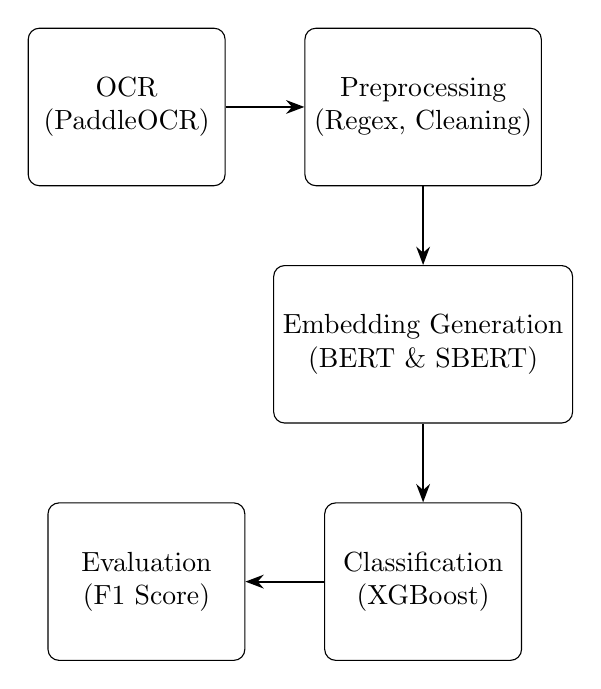
\begin{tikzpicture}[
      box/.style={
        rectangle,
        draw,
        rounded corners,
        minimum width=2.5cm,
        minimum height=2cm,
        align=center
      },
      >={Stealth},
      every edge/.style={draw, thick, -{Stealth}},
      node distance=1cm
    ]
    % Nodes
    \node[box] (ocr) {OCR\\(PaddleOCR)};
    \node[box, right=of ocr] (pre) {Preprocessing\\(Regex, Cleaning)};
    \node[box, below=of pre] (emb) {Embedding Generation\\(BERT \& SBERT)};
    \node[box, below=of emb] (clf) {Classification\\(XGBoost)};
    \node[box, left=of clf] (eval) {Evaluation\\(F1 Score)};

    % Arrows
    \path (ocr) edge (pre)
          (pre) edge (emb)
          (emb) edge (clf)
          (clf) edge (eval);
  \end{tikzpicture}
  \caption{High‐level flowchart of the receipt processing and classification pipeline}
  \label{fig:pipeline_flowchart_vertical}
\end{figure}


\section{Data Sources, Collection and Preparation}

\subsection{Data Acquisition and Annotation}
The primary dataset consists of 292 line‐item entries extracted from 26 scanned receipts using PaddleOCR. To address class imbalance,
the dataset was enriched with GPT‐generated synthetic examples, achieving a more uniform distribution across categories. Each entry was manually annotated
with a product category— according to a  8‐class schema (Food, Beverages, Snacks, Hygiene,
Housing, Healthcare, Discount, Other)—and the corresponding cost. All annotations were consolidated into a single CSV file for subsequent processing.

\subsection{Data Pipeline and Loading}
Our pipeline begins by reading the annotated CSV, which contains columns:
\begin{itemize}
  \item \textbf{Text}: Extracted text from the receipt line item.
  \item \textbf{Category}: Annotated category label (8 classes).
  \item \textbf{Cost}: Cost associated with the product.
\end{itemize}
A label encoder converts the categorical labels into numeric codes. 
To ensure consistency and reduce noise in the textual input, a set of normalization and cleaning steps was applied to each text line. 
The objective was to eliminate irrelevant artifacts and standardize the structure of the 
text prior to embedding generation and classification.

Punctuation characters were replaced with spaces to clearly separate word tokens and improve downstream tokenization. 
Consecutive whitespace characters were collapsed into a single space to maintain uniform spacing. 
Citation-like patterns were removed to eliminate non-linguistic references commonly produced by OCR.
All non-alphanumeric characters—excluding whitespace—were stripped to retain only meaningful text content. 
Numerical digits were removed to reduce the influence of context-irrelevant pricing or codes, and single-character words were  
excluded, as they typically carry little semantic value in this domain.

These preprocessing operations helped standardize the textual data and ensure that only informative content was passed to the embedding models  
and classifier.
Finally, the balanced dataset is split into training (70 \%) and test (30 \%) sets, ensuring that each
subset maintains the overall class distribution.

\subsection{Class Distribution Analysis}

Figure~\ref{fig:dist_8class} presents a comparison of two distinct datasets used in this study: the original OCR-extracted and manually  
annotated receipt data, and a supplementary dataset generated using GPT. The latter was constructed to ensure equal representation across all  
defined classes and is therefore referred to as the “balanced” GPT dataset.

In the case of the 8-class taxonomy, the original receipt data show a strong class imbalance. The \emph{Food} category dominates, comprising  
more than half of all annotated items, while other categories, such as \emph{Hygiene} or \emph{Healthcare}, are represented by only a few  
examples. This skew is expected, as food is naturally the most frequent part of daily purchases. However, such an imbalance poses a challenge  
for classification, as models trained on these data tend to favor majority classes. In contrast, the GPT-generated dataset contains  
approximately the same number of samples per class. While this is useful for introducing diversity and covering underrepresented categories,  
the uniformity of the GPT dataset does not reflect the real-world class distribution present in actual receipts.

Although balancing categories is useful during data augmentation, the use of such synthetic data for model training requires alignment with the  
distribution observed in real receipts. If the class distribution between the original and GPT datasets differs significantly, the resulting  
model may overfit to artificial class proportions rather than learning meaningful class distinctions. Therefore, prior to training, the  
GPT-generated data should be resampled to reflect the empirical class distribution of the original data.

Maintaining comparable class distributions across datasets ensures that the classifier is exposed to realistic category proportions and that  
performance comparisons are based on model effectiveness rather than artifacts of imbalanced or overly uniform training inputs.

\begin{figure}[h!]
  \centering
  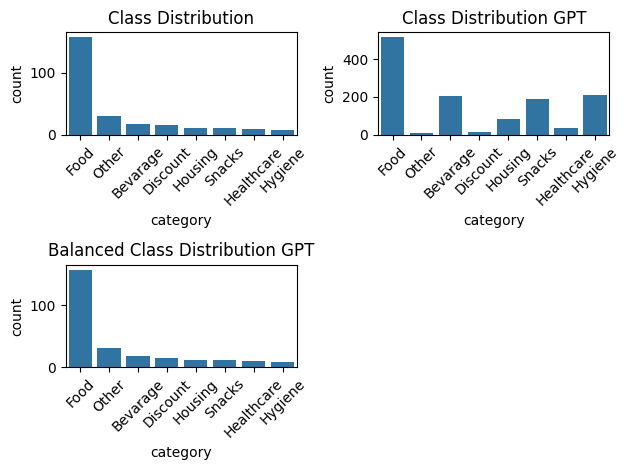
\includegraphics[width=0.8\textwidth]{images/class_distribution_8classes.png}
  \caption{Original, GPT-augmented, and balanced (bottom) class distributions.}
  \label{fig:dist_8class}
\end{figure}

\newpage
\subsection{Embedding Generation}
Two distinct embedding approaches are evaluated and compared in this study. The first utilizes the pretrained Polish BERT model 
\texttt{dkleczek/bert-base-polish-cased-v1}, which generates token-level contextual embeddings based on a broad Polish-language corpus.  
This model has not been fine-tuned for the receipt classification task and serves as a strong general-purpose baseline.

The second approach uses the \texttt{all-MiniLM-L6-v2} Sentence-BERT model, which is a lighter, sentence-level embedding model. This version has  
been further fine-tuned specifically on receipt-related data to better capture domain-specific semantics relevant to product categorization.

These two models are not used together in a single pipeline. Instead, they are compared in parallel to assess how domain adaptation and model  
size influence classification performance. In both cases, the resulting embeddings are used as input features for the XGBoost classifier.



\section{Modeling and Analysis}
This section describes the structure of the modeling experiments and the rationale behind the comparison strategy. The classification task is  
handled using the XGBoost algorithm, which operates on fixed-length vector embeddings generated from individual receipt line items. The model  
receives as input either general-purpose or fine-tuned sentence embeddings, depending on the experiment.

Two distinct embedding sources are evaluated independently. The first uses the Polish BERT model \texttt{dkleczek/bert-base-polish-cased-v1},  
which is pretrained on a general corpus and not adapted to the receipt classification task. The second approach uses the  
\texttt{all-MiniLM-L6-v2} Sentence-BERT model, which has been further fine-tuned on a domain-specific receipt dataset. These models are not  
used jointly, but rather compared in parallel to assess their effectiveness in representing receipt-level semantics.

To ensure that each model configuration performs at its best, the XGBoost hyperparameters are not fixed across experiments. Instead, the  
classifier is tuned separately for each embedding approach. Hyperparameters such as learning rate, maximum tree depth, number of estimators,  
and regularization strength are optimized individually using cross-validation on the training set. This allows each embedding–classifier  
combination to be evaluated under its most favorable settings, ensuring that the comparison reflects true model capability rather than  
differences in optimization constraints.

Classification is performed in 8-class taxonomy for both of the embedding types. In each setup, training and testing splits are kept consistent across  
experiments to allow fair comparison. Model performance is measured using the macro-averaged F1 score, which gives equal weight to each class,  
regardless of frequency. This is especially important given the underlying imbalance in real-world receipt data.

Overall, the modeling strategy is designed to evaluate how both the choice of embeddings and the label schema affect classification accuracy,  
while giving each setup the opportunity to achieve optimal performance through tailored hyperparameter tuning.


\section{Experimental Setup and Evaluation}
All experiments were managed using the Hydra framework, which provided structured configuration management and ensured reproducibility across  
runs. The training data included both the original receipt dataset and GPT-generated samples, with the latter resampled to match the class  
distribution of the original data.

Four classification scenarios were evaluated, corresponding to two embedding strategies—Polish BERT and fine-tuned Sentence-BERT—each tested  
on both the original and GPT-augmented training sets. This experimental setup enables a direct comparison of how embedding quality and data  
composition affect final model performance.

Evaluation metrics, including accuracy and macro-averaged F1 scores, are reported in Chapter~V.


\section{Summary}
The methodology presented in this chapter combines OCR-based text extraction, manual data annotation, targeted text preprocessing, and  
embedding-based feature generation with an XGBoost classifier. The experimental framework is structured to support a systematic comparison  
between two embedding strategies and to evaluate classification performance under different training conditions. This design allows for  
reliable assessment of how embedding quality and data composition influence the effectiveness of multi-class product categorization from  
receipt data.

\chapter{Implementation}

\section{Overview}

The implemented system is designed as a modular pipeline, with clearly defined components for data loading,
preprocessing, embedding generation, model training, and evaluation. Each component is developed independently
and integrated through centralized configuration management provided by Hydra.

This modular structure allows easy substitution and evaluation of different embedding methods, classification
algorithms, and data sources without requiring extensive code changes. All configurations, including
hyperparameters, dataset versions, and experimental setups, are centrally managed by Hydra, ensuring consistent
and reproducible experimentation.

Implemented entirely in Python, the system emphasizes code readability, extensibility, and reproducibility.
It supports multiple embedding models, seamlessly switching between pretrained and fine-tuned variants.
Experiment results, logs, and artifacts are systematically organized, simplifying comparison and analysis.

\section{Technology Stack}

The implementation leverages a carefully selected set of technologies and libraries to ensure robust, efficient, and scalable functionality.  
Below is an overview of the core components used in the system:

\begin{itemize}
    \item \textbf{Programming Language:} Python 3.10 was chosen due to its extensive ecosystem and strong support for machine learning, NLP, and computer vision tasks.

    \item \textbf{OCR Framework:} PaddleOCR was selected for its modular architecture, robust multilingual capabilities, and strong support for Polish text recognition.

    \item \textbf{Embedding Models:}
    \begin{itemize}
        \item \texttt{dkleczek/bert-base-polish-cased-v1} for generating general-purpose contextual embeddings in Polish.
        \item \texttt{all-MiniLM-L6-v2} Sentence-BERT model, specifically fine-tuned on receipt-related textual data.
    \end{itemize}

    \item \textbf{Classification Framework:} XGBoost was chosen for its efficiency, scalability, and consistently high performance in supervised classification tasks.

    \item \textbf{Data Processing and ML Libraries:}
    \begin{itemize}
        \item \texttt{Transformers}: Handling pretrained language models.
        \item \texttt{SentenceTransformers}: Fine-tuning and generating semantic embeddings.
        \item \texttt{scikit-learn}: Data preprocessing, evaluation metrics, and utility functions.
    \end{itemize}

    \item \textbf{Configuration Management:} Hydra framework for centralized and reproducible experiment configuration management.

    \item \textbf{Visualization Libraries:} Matplotlib and Seaborn for data visualization, exploratory analysis, and evaluating model performance.

    \item \textbf{System Dependencies:}
    \begin{itemize}
        \item \texttt{CUDA}: GPU acceleration during training and inference.
        \item \texttt{PyTorch}: Deep learning backend framework.
        \item \texttt{OpenCV}: Image preprocessing tasks, including resizing, binarization, and noise reduction.
    \end{itemize}
\end{itemize}

This technology stack was selected to balance performance, ease of integration, and extensibility, enabling reliable experimentation and reproducible outcomes.

\section{System Architecture}

The implemented system employs a modular architecture, structured into distinct components to ensure clarity, flexibility, and scalability.  
Each module is responsible for a specific task in the processing pipeline, and data flows sequentially through these interconnected modules:

\begin{itemize}
    \item \textbf{OCR Module:} Extracts textual information from scanned receipt images using PaddleOCR.
    \item \textbf{Preprocessing Module:} Cleans, normalizes, and prepares the extracted text by addressing language-specific issues such as Polish diacritics, abbreviations, and common OCR-induced errors.
    \item \textbf{Embedding Module:} Converts the preprocessed textual data into numerical embeddings, utilizing pretrained language models like Polish BERT or fine-tuned Sentence-BERT.
    \item \textbf{Classification Module:} Uses XGBoost to categorize products based on generated embeddings into predefined expense-related classes.
    \item \textbf{Evaluation Module:} Measures and assesses the classifier’s performance using metrics such as accuracy and macro-averaged F1 scores.
\end{itemize}

This modular design supports independent development, evaluation, and substitution of individual components, enabling straightforward integration of new models or processing techniques. The detailed data flow and interactions between these modules are illustrated in the "Research Design" section (Figure~\ref{fig:pipeline_flowchart_vertical}).

\section{Component Implementation}

\subsection{DataLoader and Input Handling}

The DataLoader module loads and prepares input data for further processing. It accepts CSV files containing receipt line-item texts,
annotated product categories, and associated costs. The module supports two types of input data: original OCR-extracted receipts and
GPT-generated synthetic receipts, ensuring unified preprocessing for both.

To mitigate class imbalance within the training dataset, the DataLoader implements undersampling by randomly taking samples from different
categories until they share the same distribution. This approach balances the class distribution, improving classifier performance and reducing bias
towards dominant categories.

\subsection{Preprocessing Module}

The preprocessing module is responsible for cleaning and standardizing the raw textual data obtained from the OCR output. It utilizes regular  
expressions to remove unwanted elements such as punctuation marks, numerical artifacts, and citation-like patterns. The text is then  
normalized by converting all characters to lowercase and removing redundant whitespace characters.

Additionally, specific preprocessing steps tailored to the Polish language are implemented. These include the restoration of Polish diacritics  
and the expansion of common abbreviations frequently encountered in receipts. These transformations ensure consistent formatting of text,  
facilitating effective embedding generation and subsequent classification tasks.

\subsection{Embedding Interface}

The Embedding Interface module provides a standardized mechanism for transforming preprocessed textual data into numerical vector representations.  
It integrates two embedding strategies, both leveraging pretrained transformer-based models:

\begin{itemize}
  \item \textbf{Polish BERT (\texttt{dkleczek/bert-base-polish-cased-v1}):} Generates token-level contextual embeddings suitable for capturing  
  general semantic and syntactic information.

  \item \textbf{Sentence-BERT (\texttt{all-MiniLM-L6-v2}):} Produces sentence-level semantic embeddings, specifically fine-tuned on  
  receipt-related data to capture domain-specific nuances.
\end{itemize}

Internally, the module manages:

\begin{itemize}
  \item Model initialization and loading.
  \item Tokenization using model-specific tokenizers.
  \item Batch processing for computational efficiency.
  \item Extraction and aggregation of embedding vectors.
\end{itemize}

This standardized processing ensures consistency and compatibility for downstream tasks, such as classification.

\subsection{Training and Evaluation Pipeline}

The Training and Evaluation pipeline implements supervised categorization using the XGBoost gradient boosting algorithm. Its responsibilities include:

\begin{itemize}
  \item Training the classifier using numerical embeddings as input features and annotated product categories as target labels.
  \item Splitting data into distinct training and validation subsets to facilitate effective hyperparameter optimization via cross-validation.
  \item Centralized experiment management through Hydra configuration files, specifying hyperparameters, dataset paths, and model parameters to ensure  
  reproducibility and consistency across runs.
\end{itemize}

The evaluation component computes critical performance metrics, specifically accuracy and macro-averaged F1 scores, allowing systematic and objective  
comparison across various embedding approaches and experimental configurations.

\section{Training Configuration}
The training configuration for the experiments is as follows:
\begin{itemize}
    \item \textbf{Hardware:}
    \begin{itemize}
        \item CPU: AMD Ryzen 7600
        \item GPU: NVIDIA RTX Titan
        \item RAM: 32 GB
    \end{itemize}
    \item \textbf{Software:}
    \begin{itemize}
        \item Operating System: Ubuntu 22.04
        \item Python Version: 3.10
        \item CUDA Version: 11.8
        \item PyTorch Version: 2.0
    \end{itemize}
    \item \textbf{Reproducibility:}
    \begin{itemize}
        \item Random Seed: 42 Fixed for all experiments to ensure reproducibility.
        \item Logging: All experiment logs, metrics, and configurations are stored using Hydra's output directory structure.
    \end{itemize}
    \item \textbf{Approximate Training Time:} The XGBoost classifier training is very fast and typically completes within seconds. 
    The longest process is embedding fine-tuning, 
    which takes approximately 10 to 30 minutes depending on the dataset size and model complexity.
\end{itemize}

\section{Reproducibility and Setup}

To ensure reproducibility and ease of setup, the project follows a structured organization and provides clear installation instructions.

\subsection{Project Structure}
The project is organized as follows:
\begin{itemize}
    \item \textbf{src/}: Main Python package  
    \begin{itemize}
        \item \textbf{analysis/}: Jupyter notebooks for exploratory data analysis, visualization, and prototyping (e.g.\ \texttt{data\_analysis.ipynb}, \texttt{thesis\_visualization.ipynb}, \texttt{tokenization.ipynb}).  
        \item \textbf{conf/}: Hydra configuration files and parameter definitions  
        \begin{itemize}
            \item \texttt{config.yaml}  
            \item \texttt{params/}\,(additional YAML fragments)  
        \end{itemize}
        \item \textbf{data/}: Code-organized data and annotations  
        \begin{itemize}
            \item \texttt{annotations/}  
            \item \texttt{images/}  
        \end{itemize}
        \item \textbf{model/}: Model code and artifacts  
        \begin{itemize}
            \item \texttt{dataloader.py}, \texttt{classifier.py}, \texttt{embeddings.py}, \texttt{ocr.py}  
            \item \texttt{xgboost\_model.json}  
        \end{itemize}
        \item \textbf{scripts/}: Stand-alone Python scripts (e.g.\ \texttt{annotation\_pipeline.py}, etc.)  
        \item \textbf{utils/}: Utility functions and helpers (\texttt{utils.py})  
    \end{itemize}

    \item \textbf{main.py}, \textbf{train\_model.py}: Top-level entry points for running the pipeline and training the model.

    \item \textbf{pyproject.toml}, \textbf{uv.lock}: Project metadata and locked dependencies for UV.

    \item \textbf{README.md}, \textbf{.gitignore}: Project documentation and Git ignore rules.
\end{itemize}

\subsection{Installation Instructions}
Follow these steps to set up the environment and reproduce the experiments:
\begin{enumerate}
    \item Install UV (Ultrafast Virtualenv) if not already installed:
    \begin{lstlisting}[language=bash]
curl -LsSf https://astral.sh/uv/install.sh | sh
    \end{lstlisting}

    \item Install dependencies for an existing project:
    \begin{lstlisting}[language=bash]
cd /path/to/project
uv sync
    \end{lstlisting}
    This reads your committed \texttt{uv.lock} (or \texttt{pyproject.toml}) and creates/populates \texttt{.venv/} automatically.

    \item Ensure CUDA is installed for GPU acceleration:
    \begin{lstlisting}[language=bash]
nvcc --version
    \end{lstlisting}
    Verify that the installed CUDA version matches the PyTorch version.

    \item Run experiments using Hydra configuration files:
    \begin{lstlisting}[language=bash]
uv run python scripts/train.py -- --config-name=config.yaml
    \end{lstlisting}
    (\texttt{uv run} will auto-sync your environment before executing.)
\end{enumerate}

These steps and details ensure that the experiments can be reproduced reliably on similar hardware and software configurations.

\subsection{Configuration Management with Hydra}

To ensure reproducibility and maintain a clean separation between code and experiment settings, all configurations were managed using the  
Hydra framework. This allowed for flexible modification of parameters such as model type, data sources, embedding strategies, and training  
hyperparameters, without changing the core implementation.

Each experiment was launched with a dedicated YAML configuration file. An example configuration is shown below:

\begin{lstlisting}[language=yaml, caption=Sample Hydra configuration]
params:
  learning_rate: 0.1
  max_depth: 6
  n_estimators: 100
  subsample: 0.8
  colsample_bytree: 0.8
  min_child_weight: 5
  gamma: 0.1
  reg_alpha: 0.1
  reg_lambda: 0.1

embeddingmodel: 'bert'
finetune: False
gptdatapath: '/path/to/gpt_generated_data8classes.csv'
datapath: '/path/to/annotations_8classes.csv'

defaults:
  - params: params_best_8classes
  - override hydra/sweeper: optuna
\end{lstlisting}

Hydra automatically stores every run in a separate output directory, including:
\begin{itemize}
  \item a full copy of the configuration used,
  \item all generated logs,
  \item result metrics.
\end{itemize}

This structure guarantees reproducibility and simplifies tracking the performance of different model configurations over multiple experiments.

\section{Summary}

The implemented system adopts a modular architecture consisting of independent components for OCR, preprocessing,
embedding generation, classification, and evaluation. This modularity enables flexible experimentation and easy
integration of alternative models or techniques. Configuration management with Hydra ensures reproducibility,
simplifies hyperparameter tuning, and supports structured comparisons across different experimental setups.

\chapter{Evaluation and Results}
\section{Experimental Setup}

To optimize model performance, a hyperparameter search was conducted using the \textbf{Optuna} framework with \textbf{1000 trials}. 
The goal was to maximize the overall F1 Score on the test set. The search space covered key parameters of the XGBoost classifier and 
included additional categorical choices related to embeddings, data and model configuration. 
Sampling was performed using TPE Sampler with seed set to 42.
The parameter values considered were:
\begin{itemize}
    \item \textbf{learning\_rate}: \{0.01, 0.05, 0.1, 0.2, 0.3\}
    \item \textbf{max\_depth}: \{3, 5, 7, 10, 15, 20\}
    \item \textbf{n\_estimators}: \{50, 100, 200, 300, 500, 750, 1000\}
    \item \textbf{subsample}: \{0.5, 0.6, 0.7, 0.8, 0.9, 1.0\}
    \item \textbf{colsample\_bytree}: \{0.5, 0.6, 0.7, 0.8, 0.9, 1.0\}
    \item \textbf{min\_child\_weight}: \{1, 2, 3, 5, 7, 10\}
    \item \textbf{gamma}: \{0.0, 0.1, 0.5, 1.0, 2.0, 5.0\}
    \item \textbf{reg\_alpha}: \{0.0, 0.1, 0.5, 1.0, 2.0, 5.0\}
    \item \textbf{reg\_lambda}: \{0.0, 0.1, 0.5, 1.0, 2.0, 5.0\}
    \item \textbf{embeddingmodel.model\_path}: \{mini\_finetuned\_base, mini\_finetuned\_augmented, bert\}
    \item \textbf{augument\_classifier}: \{True, False\}
    \item \textbf{balance\_data}: \{True, False\}
\end{itemize}

This setup enabled the optimization process to explore a broad range of configurations in a structured and efficient way. 
Although the sampler could occasionally converge to local optima, 
overall model performance improved substantially through hyperparameter fine-tuning and selection of the best-performing configuration.

\section{Evaluation Metrics}

To evaluate model performance, standard metrics are used: accuracy, precision, recall, and F1 score. Accuracy reflects the overall proportion  
of correct predictions but can be misleading in imbalanced datasets. Precision and recall offer a more detailed view—precision measures how  
many predicted positives are correct, while recall indicates how many actual positives are captured.

The main evaluation metric in this study is the micro-averaged F1 score, also referred to as the overall F1 score. It aggregates true positives,  
false positives, and false negatives across all classes and is particularly appropriate when class imbalance exists, as it reflects the model’s  
global effectiveness.

In addition to this, macro-averaged F1 score is reported. It calculates F1 scores per class and averages them, giving equal weight to all  
categories. This provides insight into the model’s balance across both frequent and rare classes.

Reporting both micro and macro F1 scores allows for fair evaluation: the former captures overall performance, while the latter highlights how  
well the model handles less-represented categories.


\section{Result Analysis}
\subsection{Best Performing Model}

The best results were achieved using the \texttt{all-MiniLM-L6-v2} model from the Sentence-Transformers library. This embedding model was  
fine-tuned exclusively on real receipt data, without using any GPT-generated examples during the embedding stage. The final classification was  
performed using an XGBoost model trained on a combination of real and GPT-augmented data. The GPT samples were balanced across classes to improve  
generalization on underrepresented categories.

This configuration achieved an overall accuracy of 79.55\%, a micro-averaged (overall) F1 score of 0.8053, and a weighted F1 score of 0.81.  
The macro-averaged F1 score reached 0.70, confirming strong and consistent performance across both frequent and rare classes.

\subsubsection*{Model Configuration}

The XGBoost classifier was tuned using the following hyperparameters:

\begin{itemize}
  \item \texttt{learning\_rate}: 0.01 \quad \texttt{max\_depth}: 5 \quad \texttt{n\_estimators}: 1000
  \item \texttt{subsample}: 1.0 \quad \texttt{colsample\_bytree}: 0.7
  \item \texttt{min\_child\_weight}: 2 \quad \texttt{gamma}: 2.0
  \item \texttt{reg\_alpha}: 0.0 \quad \texttt{reg\_lambda}: 5.0
\end{itemize}

\subsubsection*{Overall Performance}

The performance summary for this configuration is presented in Table~\ref{tab:best_model_summary}. The model demonstrates strong micro and macro  
F1 scores, making it the most balanced configuration tested. It also confirms that fine-tuning the embedding model on domain-specific real data  
is more effective than relying on pretrained models alone.

\begin{table}[h!]
  \centering
  \caption{Overall performance – Best model (\texttt{all-MiniLM-L6-v2} fine-tuned on real data, XGBoost trained on real + GPT-balanced data)}
  \label{tab:best_model_summary}
  \begin{tabularx}{\textwidth}{lccc}
    \toprule
    \textbf{Metric}         & \textbf{Macro Average} & \textbf{Weighted Average} & \textbf{Overall Accuracy} \\
    \midrule
    Precision               & 0.74                   & 0.83                      & 0.7955 \\
    Recall                  & 0.70                   & 0.80                      & 0.7955 \\
    F1 Score (Macro)        & 0.70                   & 0.81                      & 0.7955 \\
    F1 Score (Micro)        & \multicolumn{3}{c}{0.8053} \\
    Overall Accuracy  & \multicolumn{3}{c}{0.7955} \\
    \bottomrule
  \end{tabularx}
\end{table}

\subsubsection*{Class-Level Performance}

The detailed classification report is shown in Table~\ref{tab:best_model_report}. High F1 scores are achieved for the dominant classes  
\emph{Food} (0.88), \emph{Discount} (0.91), and \emph{Beverage} (0.83). These categories benefit from strong representation in the dataset (Food)
or consistent linguistic patterns (Discount,Bevarage). More challenging classes like \emph{Housing} and \emph{Healthcare} achieved moderate performance (F1 = 0.50  
and 0.47 respectively).

\begin{table}[h!]
  \centering
  \caption{Full classification report – Best model}
  \label{tab:best_model_report}
  \begin{tabularx}{\textwidth}{lcccc}
    \toprule
    \textbf{Class} & \textbf{Precision} & \textbf{Recall} & \textbf{F1 Score} & \textbf{Support} \\
    \midrule
    Beverages (0)     & 1.00 & 0.71 & 0.83 & 7 \\
    Discount (1)      & 1.00 & 0.83 & 0.91 & 6 \\
    Food (2)          & 0.89 & 0.87 & 0.88 & 55 \\
    Healthcare (3)    & 0.36 & 0.67 & 0.47 & 6 \\
    Housing (4)       & 0.50 & 0.50 & 0.50 & 4 \\
    Other (5)         & 0.67 & 0.60 & 0.63 & 10 \\
    \midrule
    \textbf{Macro Avg}         & 0.74  & 0.70  & 0.70 & 88 \\
    \textbf{Weighted Avg}      & 0.83  & 0.80  & 0.81 & 88 \\
    \textbf{Overall Accuracy}  & \multicolumn{4}{c}{0.7955} \\
    \textbf{Micro Avg F1 Score}& \multicolumn{4}{c}{0.8053} \\
    \bottomrule
  \end{tabularx}
\end{table}

In summary, this configuration provides the most balanced and robust performance. Fine-tuning the embedding model exclusively on real data  
appears to preserve domain-specific semantics, while the use of GPT-balanced data for classifier training helps correct for class imbalance.  
This model sets a reliable benchmark for further improvements in receipt-based product categorization.

\subsection{Fine-Tuned Sentence-Transformer on Mixed Data}

This configuration used the \texttt{all-MiniLM-L6-v2} model fine-tuned on a combination of real and GPT-augmented data. The XGBoost classifier,  
however, was trained only on real receipt data. This setup achieved an accuracy of 78.41\%, a weighted F1 score of 0.80, and a macro-averaged  
F1 score of 0.77. Although the overall (micro) F1 score was slightly lower (0.7967) than the best-performing model, the macro-average indicates  
better class-wise consistency mostly due to high improvemend in Healthcare class

\begin{table}[h!]
  \centering
  \caption{Full classification report – Sentence-Transformer fine-tuned on real + GPT data, XGBoost trained on real data}
  \label{tab:finetuned_st_real_clf_report}
  \begin{tabularx}{\textwidth}{lcccc}
    \toprule
    \textbf{Class} & \textbf{Precision} & \textbf{Recall} & \textbf{F1 Score} & \textbf{Support} \\
    \midrule
    Beverages (0)     & 0.88 & 1.00 & 0.93 & 7 \\
    Discount (1)      & 1.00 & 0.83 & 0.91 & 6 \\
    Food (2)          & 0.88 & 0.78 & 0.83 & 55 \\
    Healthcare (3)    & 1.00 & 0.83 & 0.91 & 6 \\
    Housing (4)       & 0.50 & 0.50 & 0.50 & 4 \\
    Other (5)         & 0.41 & 0.70 & 0.52 & 10 \\
    \midrule
    \textbf{Macro Avg}         & 0.78 & 0.77 & 0.77 & 88 \\
    \textbf{Weighted Avg}      & 0.82 & 0.78 & 0.80 & 88 \\
    \textbf{Overall Accuracy}  & \multicolumn{4}{c}{0.7841} \\
    \textbf{Micro Avg F1 Score}& \multicolumn{4}{c}{0.7967} \\
    \bottomrule
  \end{tabularx}
\end{table}

This model shows better macro-averaged F1 performance compared to others, reflecting more balanced results across all classes, including  
underrepresented ones.

\subsection{BERT-Based Model (Out-of-the-Box)}

This experiment evaluates the performance of the pretrained Polish BERT model (\texttt{dkleczek/bert-base-polish-cased-v1}) used without  
task-specific fine-tuning. Despite its significantly larger architecture compared to \texttt{all-MiniLM-L6-v2}, the model achieves lower performance across  
key metrics and slower inference speed, making it a less practical choice in this context.

The model reached an accuracy of 72.73\% and a weighted F1 score of 0.7073. While these values are comparable to other configurations, the  
macro-averaged F1 score dropped to 0.51—substantially lower than previous model. This decline highlights  
its inability to generalize well across all classes, especially those with lower support or more semantic variability.

As expected, the \emph{Food} category continues to dominate in terms of recall (0.89) and F1 score (0.83). However, several other classes exhibit  
weaker performance. For instance, the \emph{Beverage} class yields an F1 score of only 0.18, while the \emph{Housing} class is not predicted  
correctly at all. These issues result in poor macro-averaged metrics, confirming that the model disproportionately favors majority classes and  
struggles with semantically diverse or underrepresented labels.

It is also important to emphasize the inefficiency of this model. BERT’s size significantly increases inference time without offering a  
performance advantage. In contrast, the smaller \texttt{all-MiniLM-L6-v2}, fine-tuned on receipt data, achieves superior scores  
 while delivering much faster predictions—making it a more suitable choice for real-world applications.

A full classification breakdown for this BERT configuration is provided in Appendix~\ref{appendix:bert-report-outofbox}.


\chapter{Discussion}

\section{Interpretation of Results}

Table~\ref{tab:results_comparison} summarizes and compares the three evaluated
configurations. The best-performing setup (0.81 micro-F1) utilizes the 
\texttt{all-MiniLM-L6-v2} embedding model fine-tuned solely on real receipt data, 
paired with an XGBoost classifier trained on combined real and GPT-augmented 
datasets. The mixed-data embedding fine-tuning achieves a higher macro-F1 score 
(0.77), reflecting more balanced classification performance across categories, 
particularly improving classes such as \emph{Healthcare}. The out-of-the-box Polish 
BERT model performs poorly across all metrics, also incurring a substantial inference 
time penalty.

\begin{table}[h!]
  \centering
  \caption{Performance comparison of the evaluated model pipelines}
  \label{tab:results_comparison}
  \begin{tabularx}{\textwidth}{lcccX}
    \toprule
    \textbf{Pipeline} & \textbf{Accuracy} & \textbf{F1\textsubscript{micro}}
                      & \textbf{F1\textsubscript{macro}} & \textbf{Main findings} \\
    \midrule
    MiniLM (real) + XGBoost (real+GPT) & 0.80 & 0.81 & 0.70 &
      Best overall accuracy; GPT augmentation improves minority-class recall. \\
    MiniLM (real+GPT) + XGBoost (real) & 0.78 & 0.80 & 0.77 &
      Highest macro-F1; balanced across classes, notably enhanced \emph{Healthcare}. \\
    BERT (pre-trained) + XGBoost (real) & 0.73 & 0.71 & 0.51 &
      Slow inference; weak generalization, favors majority class (\emph{Food}). \\
    \bottomrule
  \end{tabularx}
\end{table}

\subsection{Impact of fine-tuning.} Domain-specific fine-tuning proves more 
effective than using larger but unadapted models. Both MiniLM variants significantly 
outperform the larger BERT model used without fine-tuning.

\subsection{Influence of GPT augmentation.} Differences between augmentation strategies 
suggest distinct effects:

\begin{itemize}
  \item Fine-tuning embeddings on combined real and GPT data likely shifts the 
  embedding representations toward the GPT-generated distribution. Thus, introducing 
  more GPT samples at the classifier training stage could adversely affect performance 
  on real receipt examples due to mismatched data distributions.
  \item Fine-tuning embeddings exclusively on real receipt data maintains a stable 
  representation space for genuine receipt semantics. In this scenario, adding balanced 
  GPT data at the classifier stage enhances generalization without negatively affecting 
  the embedding manifold, thus benefiting overall model performance.
\end{itemize}

\subsection{Comparison of Micro and macro metrics.} The optimal configuration demonstrates the 
highest micro-F1, emphasizing accurate predictions aligned with user-visible 
performance. The mixed-data fine-tuning setup leads in macro-F1, showcasing improved 
classification balance across diverse categories.

\subsection{Practical implications.} Compact, domain-fine-tuned models such as MiniLM 
offer high accuracy and significantly faster inference times than large, general-purpose 
models. Model choice ultimately depends on practical requirements: prioritize the best 
model for maximal overall accuracy, or prefer the mixed-data configuration when 
balanced performance across classes is crucial.


\section{Recommendations for Future Work.}
Further research should focus on deeper analysis of the embedding space, exploring how
receipt semantics are represented within the embedding manifold. Visualizations and clustering
techniques could help identify semantic overlaps and areas where the embedding quality can
be improved. Additionally, incorporating a larger and more diverse set of real-world receipt
data would likely enhance generalization and robustness, particularly for minority classes
that are currently underrepresented. Such expanded datasets would facilitate more
effective fine-tuning and model optimization, potentially driving further performance gains.

\section{Limitations of the Study}

Although the presented approach achieves strong overall performance, there are several notable limitations.  
First, the primary dataset used for training and evaluation is limited in size, comprising only 20 receipts and a total of 263 items.  
This relatively small and specific dataset restricts the diversity and representativeness of the training examples, potentially affecting the generalization capability of the models, especially for infrequent or rare categories.

Second, despite the introduction of GPT-generated data to mitigate class imbalance, significant disparity in class representation remains.  
The dominance of certain categories such as \emph{Food} mirrors real-world scenarios but poses challenges to reliably classify minority categories, as synthetic data might not perfectly capture real-world variability and semantics.
Lastly, the evaluation exclusively utilized Polish-language receipts.  
Consequently, the applicability and performance of the developed system in other linguistic or regional contexts remain unverified, limiting generalizability and transferability of these findings.

Addressing these issues in future research would further enhance the robustness and applicability of the developed models.


\chapter{Conclusion}

\section{Summary of Findings}
This research highlights several key findings regarding embedding methods and data augmentation for receipt  
classification tasks. Fine-tuning the Sentence-Transformer embedding model (\texttt{all-MiniLM-L6-v2})  
exclusively on real-world receipt data resulted in the highest overall (micro) F1 score of 0.81, emphasizing  
the importance of domain-specific embedding adaptation. Incorporating GPT-generated synthetic data at the  
classifier training stage significantly improved generalization and particularly enhanced predictions for  
minority classes. However, directly fine-tuning embeddings on mixed GPT and real data slightly reduced overall  
accuracy, although it increased class-wise balance (macro-averaged F1 score of 0.77).  

Despite its larger architecture, the pretrained Polish BERT model \newline (\texttt{dkleczek/bert-base-polish-cased-v1}),  
used without task-specific fine-tuning, consistently underperformed, reinforcing the necessity of targeted,  
domain-specific model adaptation rather than relying solely on raw model size. Class imbalance was a consistent  
challenge: the dominant category \emph{Food} consistently achieved high scores (F1 up to 0.88), while minority  
categories such as \emph{Housing} and \emph{Healthcare} showed improved performance with GPT augmentation but  
remained difficult due to inherent semantic variability and limited training samples.

Finally, practical considerations indicated that compact, domain-specific fine-tuned embedding models offered  
both higher accuracy and faster inference compared to large, generic transformer models, thus making them  
preferable for real-world applications. These results collectively emphasize the value of domain-specific  
fine-tuning, careful synthetic data augmentation, and efficiency considerations when deploying NLP-based  
classification pipelines.


\section{Contributions to the Field}

This thesis provides several important contributions to the area of Natural Language Processing and  
receipt-based product categorization. Firstly, it presents a specialized end-to-end classification pipeline  
specifically tailored to Polish-language receipts, addressing a practical gap in existing personal finance  
management tools. Secondly, this research offers valuable insights into embedding-model strategies,  
demonstrating the significant advantages of domain-specific fine-tuning over using large pretrained models.  

Additionally, this study thoroughly examines the role of GPT-generated synthetic data, clearly illustrating  
its effectiveness in addressing class imbalance issues within receipt classification tasks. By systematically  
benchmarking different embedding and classification approaches, the thesis provides a clear comparative analysis  
and establishes robust performance benchmarks for future research. Finally, by evaluating practical aspects such  
as computational efficiency and inference speed, the research delivers actionable recommendations for effective  
and efficient real-world implementations of NLP-based categorization systems.

\chapter{Appendices}

\section{Example Receipt and Annotation}

Figure~\ref{fig:sample_receipt} presents an example receipt image used as an input for the OCR and annotation process.

\begin{figure}[h!]
    \centering
    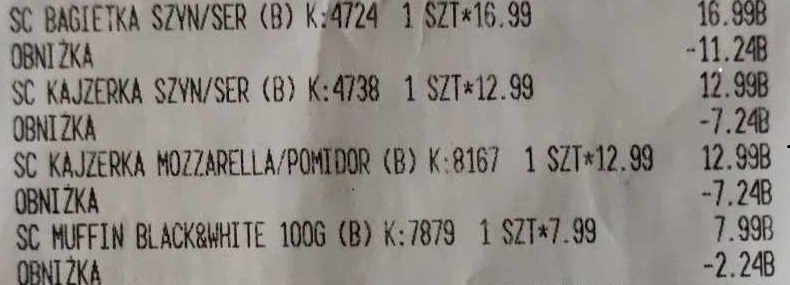
\includegraphics[width=0.6\textwidth]{images/sample_receipt.jpg}
    \caption{Sample receipt image}
    \label{fig:sample_receipt}
\end{figure}

After applying OCR (using PaddleOCR), the textual output was manually annotated with category labels and associated costs.  
Below is an example of annotated receipt data in CSV format:

\begin{verbatim}
"SC BAGIETKASZYN/SER BK47241SZT*16.9S 16.99B",Food,16.99
"OBNIZKA -11.24B",Discount,11.24
"SCKAJZERKASZYN/SERBK:47381SZT*12.99 12.99B",Food,12.99
"OBNIZKA -7.248",Discount,7.24
"SC KAJZERKA MOZZARELLA/POMIDOR (B)K81671 SZT*12.99 12.99B",Food,12.99
"OBNIZKA -7.248",Discount,7.24
"SC MUFFIN BLACK&WHITE100G BK:78791SZT*7.99 7.99B",Food,7.99
"OBNIZKA -2.24B",Discount,2.24
\end{verbatim}

This structured textual data serves as input for subsequent preprocessing, embedding generation, and classification steps detailed in earlier sections.


\section{Implementation Examples}

\subsection{Text Preprocessing}

The following example shows a text normalization function used after OCR extraction to reduce noise and standardize textual data:

\begin{lstlisting}[language=Python, caption={Post-OCR text preprocessing}, label={lst:preprocessing}]
def preprocess_text(text):
    text = re.compile('[%s]' % re.escape(string.punctuation)).sub(' ', text)
    text = re.sub(r'\s+', ' ', text)
    text = re.sub(r'[^\w\s]', '', text.strip())
    text = re.sub(r'\d', ' ', text)
    text = re.sub(r'\s*\b[a-zA-Z]\b\s*', ' ', text).strip()
    return text
\end{lstlisting}
\label{code:preprocessing_example}

This preprocessing step standardizes the extracted OCR text by removing punctuation, numbers, single characters, and excessive whitespace, thus improving subsequent embedding quality.

\subsection{OCR Pipeline}

Below is an example of PaddleOCR implementation and extraction of preprocessed data from image files:

\begin{lstlisting}[language=Python, caption={OCR class}, label={lst:ocr}]
class OCR:
    def __init__(self):
        self.paddleocr = PaddleOCR(
            use_angle_cls=True, lang='pl',
            rec_algorithm='CRNN', rec_char_type='pl'
        )

    def get_preprocessed_data(self, img_path):
        ocr_data = self.perform_ocr(img_path)
        preprocessed = []
        for line in ocr_data:
            for word_info in line:
                text = preprocess_text(word_info[1][0])
                cost = preprocess_cost(word_info[1][0])
                preprocessed.append((text, cost))
        return preprocessed
\end{lstlisting}
\label{code:ocr_pipeline_example}

This OCR pipeline leverages PaddleOCR to extract textual content from images, applying preprocessing steps to ensure high-quality inputs for further analysis.

\subsection{Sentence-Transformer Fine-tuning}

The example below demonstrates how the Sentence-Transformer embedding model (\texttt{all-MiniLM-L6-v2}) was fine-tuned using contrastive loss to better capture domain-specific semantics:

\begin{lstlisting}[language=Python, caption={Fine-tuning Sentence-Transformer embeddings}, label={lst:embedding_finetuning}]
model.fit(
    train_objectives=[(train_dataloader, loss)],
    evaluator=evaluator,
    epochs=epochs,
    warmup_steps=warmup_steps,
    evaluation_steps=len(train_dataloader),
    output_path=path,
    save_best_model=True,
)
\end{lstlisting}
\label{code:finetuning_example}

Fine-tuning was performed using labeled pairs of receipt texts to ensure embeddings accurately reflect semantic differences relevant to categorization tasks.

\subsection{Hydra-driven Model Training Pipeline}

The Hydra framework was utilized for structured experimentation, enabling easy parameter adjustments and reproducibility:


\begin{lstlisting}[language=Python, caption={Training pipeline}, label={lst:preprocessing}]
@hydra.main(config_path="./conf", config_name="config")
def main(cfg):
    dataloader = Dataloader(Path(cfg.datapath))
    embedding_model = Embedding.load_mini_model(cfg.embeddingmodel.model_path)

    train_batch, test_batch, _ = dataloader.get_training_ready_data(
        embedding_model, split_size=cfg.split_size
    )

    model = XGBoost(**cfg.params)
    model.fit(train_batch['embeddings'], train_batch['category'])
    results = model.test_model(test_batch['embeddings'], test_batch['category'])

    hydra.utils.log.info(f'Test F1 Score: {results["f1_score"]}')
\end{lstlisting}
\label{code:hydra_pipeline_example}

Using Hydra streamlined experimentation, provided automated logging of parameters and results, and ensured experimental reproducibility.



\section{Additional Figures and Tables}
\subsection{XGBoost Hyperparameters by Model Type}

\noindent The hyperparameters used for the XGBoost classifier differ slightly depending on the embedding configuration.
Below are the tuned values for each scenario.

\begin{lstlisting}[language=yaml, caption={XGBoost hyperparameters – BERT model}, label={lst:bert_params}]
learning_rate: 0.3
max_depth: 5
n_estimators: 50
subsample: 0.8
colsample_bytree: 1.0
min_child_weight: 5
gamma: 0.1
reg_alpha: 0.0
reg_lambda: 0.0
\end{lstlisting}

\begin{lstlisting}[language=yaml, caption={XGBoost hyperparameters – Sentence-Transformer (GPT + real fine-tuned)}, label={lst:gpt_real_params}]
learning_rate: 0.2
max_depth: 7
n_estimators: 500
subsample: 0.5
colsample_bytree: 0.6
min_child_weight: 7
gamma: 0.0
reg_alpha: 0.0
reg_lambda: 0.0
\end{lstlisting}

\begin{table}[h!]
  \centering
  \caption{Full classification report – BERT model (out-of-the-box, no fine-tuning)}
  \label{appendix:bert-report-outofbox}
  \begin{tabularx}{\textwidth}{lcccc}
    \toprule
    \textbf{Class} & \textbf{Precision} & \textbf{Recall} & \textbf{F1 Score} & \textbf{Support} \\
    \midrule
    Beverages (0)     & 0.25 & 0.14 & 0.18 & 7 \\
    Discount (1)      & 1.00 & 0.67 & 0.80 & 6 \\
    Food (2)          & 0.78 & 0.89 & 0.83 & 55 \\
    Healthcare (3)    & 0.50 & 0.67 & 0.57 & 6 \\
    Housing (4)       & 0.00 & 0.00 & 0.00 & 4 \\
    Other (5)         & 0.86 & 0.60 & 0.71 & 10 \\
    \midrule
    \textbf{Macro Average}   & 0.56 & 0.49 & 0.51 & 88 \\
    \textbf{Weighted Average}& 0.71 & 0.73 & 0.71 & 88 \\
    \textbf{Overall Accuracy}& \multicolumn{4}{c}{0.7273} \\
    \textbf{Overall F1 Score}& \multicolumn{4}{c}{0.7073} \\
    \bottomrule
  \end{tabularx}
\end{table}
\renewcommand{\bibname}{Bibliography}

\printbibliography

\beforelastpage

\end{document}
